\section{System Overview}
Frequent incremental maintenance of materialized views can be costly or infeasible given system constraints. 
We propose approximate query correction to address this problem, and to give a flexible tradeoff between query accuracy and system performance.
The key idea is that given a stale aggregation query (SUM, COUNT, AVG, VAR) on a materialized view, we use a sample of up-to-date data to estimate how much that data changes the stale aggregation query.
From the sample, we can derive a correction to the stale query result, which in expectation is accuracte, but has variance inherrent to sampling.

Our proposed system will work in conjunction with existing maintenance or re-calculation approaches.
We envision the scenario where materialized views are being refreshed periodically eg. nightly.
While maintaining the entire view throughout the day may be infeasible, sampling allows the database to scale maintenance with the performance and resource constraints during the day.
Then, between maintenance periods, we can provide approximately up-to-date query results for aggregation queries.

However, a challenge is that supporting only aggregation queries has the potential mask outliers in the updates.
Since, we can answer selection queries on the view, we may miss outlier rows either because they were not sampled or because
they are averaged into an aggregation query.
We define an ``outlier index" on the base table which indexes records with abnormal attribute values, where abnormality is defined by user specified rules.
Therefore, we couple our sampling with outlier indexing to guarantee that rows in the materialized views derived outlier base table records are in the sample.
The result is that we can answer selection queries exactly on these outlier rows which are often the most queried rows in the materialized view.
What is particularly surprising is that outliers can give valuable information about the data distribution and these can be used to improve the accuracy of our aggregation queries as well.

To illustrate our approach, we use the following running example which is a 
simplified schema of one of our experimental datasets (Figure \ref{example}).
Imagine, we are querying logs from a video streaming company. 
These logs record visits from users as they happen and grow over time.
We have two table: Log and Video, with the following schema:
\begin{lstlisting}
Log(sessionID, videoID, responseTime, userAgent)
Video(videoID, title, duration)
\end{lstlisting}
These tables are related with a foreign-key relationship between
Log and Video, and there is an integrity constraint that every log
record must link to one video in the video table.

\begin{figure}[h]
\label{example}
\centering
 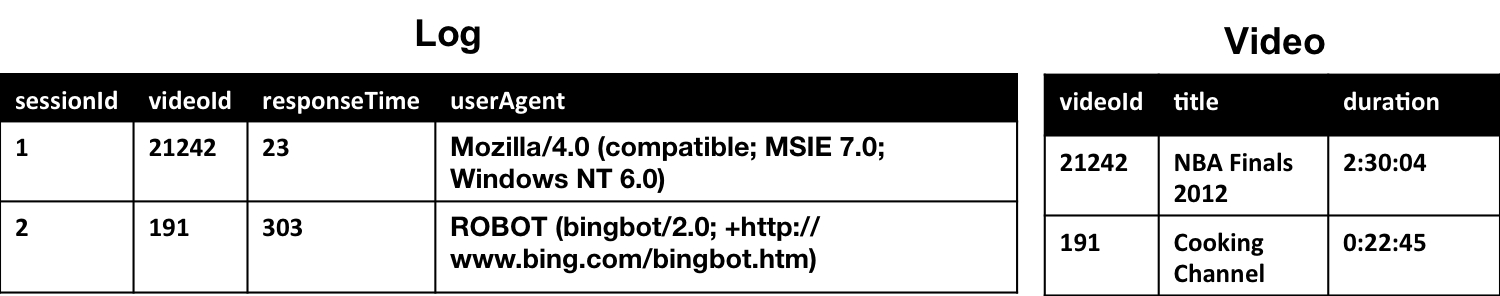
\includegraphics[width=\columnwidth]{figs/sample-clean-example.png}
 \caption{TODO}
\end{figure}

\subsection{System Architecture}
The architecture of our proposed solution is shown in Figure \ref{sys-arch}.
The left side of the diagram resembles a tradition view maintenance architecture.
However, there are a couple of key additions: (1) instead of maintaining the view,
we issue corrections to query results on the view, (2) to acheive this we maintain
an up-to-date sample, and (3) we have an outlier index.
In this section, we will overview these three components and contrast our approach 
to other materialized view and AQP architectures.

\begin{figure}[h]
\label{sys-arch}
\centering
 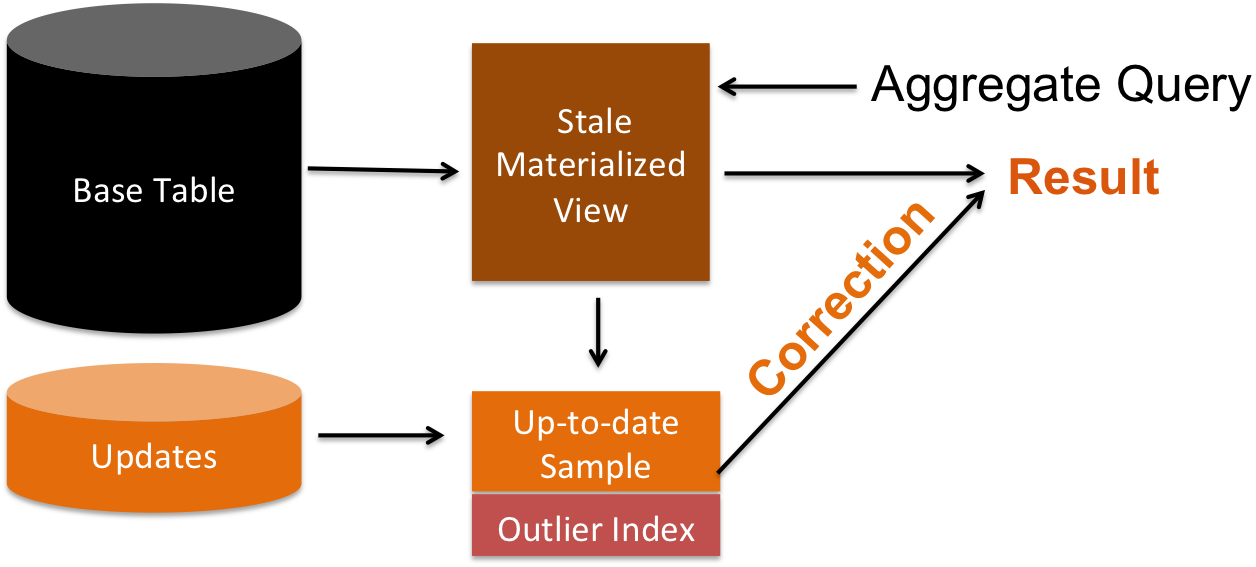
\includegraphics[width=\columnwidth]{figs/sys-arch.png}
 \caption{TODO}
\end{figure}

\subsubsection{Supported Materialized Views}\label{subsubsec:supported-view}
We will first introduce the taxonomy of materialized views
that can benefit from our approach. In particular, we provide example
situations when view maintenance can be costly. 

\vspace{1em}

\noindent\textbf{Select-Project Views}

One type of view that we consider are views generated from Select-Project
expressions of the following form:

\begin{lstlisting}
SELECT [col1,col2,...] 
FROM table 
WHERE condition([col1,col2,...]) 
\end{lstlisting}

There are situations when such views are expensive to maintain. For
example, as often the case with activity logs, the base table may
contain semi-structured data that requires parsing or preprocessing
as a part of the view definition. Consider the following example,
a typical column in online activity logs is the User-Agent String
(Figure ?). When a user accesses a webpage the browser reports this
string to identify the browser type, operating system, and layout
engine. Suppose, we wanted to create the following view:

\begin{lstlisting}
SELECT * FROM Log 
WHERE userAgent 
LIKE '%Mozilla%'
\end{lstlisting}

This involves evaluating regular expression on the string to see if
it matches a criteria.
Testing a complex regular expression will be far more expensive than
numerical comparisions or equality testing. In more extreme examples,
the columns may be serialized objects (eg. represented in JSON) which
need to be deserialized before evaluating a predicate.

%\begin{figure}
%\includegraphics[scale=0.3]{Documents/Research/sigmod15/Images/user-agent}

%\caption{User-Agent Activity Logs. <TODO>}
%\end{figure}

\vspace{1em}

\noindent\textbf{Aggregation Views}

We also consider aggregation views of the following form:

\begin{lstlisting}
SELECT [f1(col1),f2(col2),...] 
FROM table 
WHERE condition([col1,col2,...]) 
GROUP BY [col1,col2,...]
\end{lstlisting}

While the same costs that Select-Project views can incur due to pre-process
apply as well, aggregation views pose additional challenges to incremental
view maintenance. Aggregation views can be costly to maintain when
the cardinality of the result is large; that is when there group by
clause is very selective. Consider the following example:

\begin{lstlisting}
SELECT videoID, 
max(responseTime) AS maxResponseTime 
FROM Log 
GROUP BY videoID;
\end{lstlisting}

The cardinality of the delta view is the total number of videos in the log which can be very large.
Thus it will be costly to propagate this result with the existing view, potentially updating a large number of rows. 
These costs increase in a distributed environment where a larger
delta view means that more data has to be communicated through a shuffle
operation. 

\vspace{1em}

\noindent\textbf{Foreign-Key Join Views}

The third type of view we consider are Foreign-Key Join views:

\begin{lstlisting}
SELECT table1.[col1,col2,...], 
table2.[col1,col2,...]
FROM table1, table2 
WHERE table1.fk = table2.fk 
AND condition([col1,col2,...]) 
\end{lstlisting}

Such views are ubquitious in star schemas {[}?{]} and can be particularly
costly to maintain in distributed environments. Consider the following example:

\begin{lstlisting}
SELECT * 
FROM Log, Video 
WHERE Log.videoID = Video.videoID;
\end{lstlisting}

Suppose new recrods have been inserted into Log. Calculating the
delta view involves joining the new records with the entire table Video.
While indexing is the prefered strategy to optimize such joins, many
distributed systems, such as Apache Spark, Cloudera Impala, and Apache
Tez, lack native support for join indices. To avoid scanning the entire
table, these systems rely on partitioned joins where records linked
by foreign keys are stored on the same partition. However, when these
join keys cross partition lines this operation can become increasingly
expensive.

\subsubsection{Up-to-date Samples}
We presented examples where these views can be expensive to maintain.
In this work, we address the question of whether we need to maintain
the entire view to answer aggregate queries on these views. Our proposed
solution is to sample the delta view $\Delta\textbf{V}$, and incrementally
maintain just a sample of $\textbf{V}_{T}$. For example, in our Select-Project
view example application, we would have to parse only a sample of
the inserted records. Similarly, for the Aggregation view, sampling
$\Delta\textbf{V}$ reduces the cardinality of the result and consequently
communication/merging costs. And finally, for the Join views, we would
only have to join a sample of the inserted records. 

\subsubsection{Outlier Indexing}
We are often interested in records that outliers, 
which we define in this work as records with abnormally large attribute values.
Outliers and power-law distributions are a common property in web-scale datasets.
Often the queries of interest involve the outlier records, however sampling does 
have the potential to mask outliers in the updates.
If we have a small sampling ratio, more likely than not, outliers will be missed.

Therefore, we propose coupling sampling with outlier indexing. 
That is, we guarantee that records (or rows in the view derived from those records) 
with abnormally large attribute values are included in the sample.
What is particularly interesting is that these records give information about the distribution 
and can be used to reduce variance in our estimates.

\subsubsection{Alternative Architectures}
\noindent\textbf{No Maintenance: }
One approach for up-to-date results is to avoid incremental maintenance altogether.
In this approach, one would periodically re-calculate the views.
This approach allows for the highest throughput in terms of records written, but can
suffer from long periods of stale data.

\vspace{1em}

\noindent\textbf{View Maintenance: }
The other option is to fully maintain the materialized view. 
While immediate maintenance offers consistent results, 
it is at a steep computational cost.
So often incremental maintenance, is deferred or done periodically [?].
These deferred schemes can lead to period of staleness as well.

\vspace{1em}

\noindent\textbf{SAQP: }
Estimating the results of aggregate queries from samples has been
well studied in a field called Sample-based Approximate Query Processing
(SAQP). While the concept of estimating a correction from a sample
is similar to SAQP it differs in a few critical ways. Traditional
SAQP techniques apply their sampling directly to base tables and not
on views. The SAQP approach to this problem, would be to treat aggregate
queries on views as nested queries and then apply them to a sample
of the base data {[}?{]}. Another potential technique would be to
estimate the result directly from the maintained sample; a sort of
SAQP scheme on the sample of the view. We found that empricially estimating
a correction and leveraging an existing deterministic result lead
to lower variance results on real datasets (see Section ?). We analyze
the tradeoffs of these techniques in the following sections.

\vspace{1em}

Our approach provides a flexible tradeoff between the performance benefits of No Maintenance and the Consistency benefits of full maintenance. Accordingly, we evaluate our approach against the accuracy of not maintaining the data and the performance of maintaining the data.
We further compare our approach to SAQP, configured so it would have the same cost, in terms of accuracy.